% !TEX root = main.tex
\chapter{Discussion}
  The following section will discuss the results in chapter \ref{chap:experiments} and the simulations made in chapter \ref{chap:simulations}. The purpose of this paper was to investigate the effects or aerodynamics on race cars, design a solution that would improve the car's lap time and finally produce the hypothesized aerodynamic device.

  \section{Theory, Experiments and Simulations}

  The wind tunnel results plotted in figure \ref{fig:clperAOAexperiment} shows a correlation between the wing's lift and theoretical lift, assuming a constant $C_L$ for the theoretical wing. The experimental results are all lower than the theoretical, which may be due to several facts: First, the wing section's alignment at higher speeds was interrupted, as one section was skewed $\SIrange{2}{3}{\milli\metre}$, creating a small gap between the wing sections. Secondly, the wing's extremely high lift interferes with the flow behaviour, as the wing's wake is most likely pushing air against the walls. This theory is corroborated by the simulations as seen in figure \ref{fig:scalewingwindtunnelsim}, where it is clearly seen that the wake interferes with the wall's boundary layer. Third, and most likely the most important, the placement relative to each other may be slightly off. Creating a small multi element airfoil is very difficult, as placement is everything to the lift of the wing. According to the wing optimization process seen in figure \ref{fig:multieleoptimization}, very small changes can rapidly change the  lifting characteristics of the wing. This could explain why the lift of the airfoil model is much lower than the theoretical, and the fact that the simulations coincide very well with theory.

  After evaluating the experimental results and the simulations, it was clear that theory sided with the simulations. This evoked an investigation of the down scaled wing model, revealing a relative position of the trailing-edge-to-tip position of $(x,y) = (\SI{-11.5}{\milli\metre},\SI{-8}{\milli\metre})$, instead of the planned $(\SI{-6.9}{\milli\metre},\SI{-12.5}{\milli\metre})$. The variation comes from placing the wing initially. The importance of the position was not uncovered until simulations optimizing their relative position, and due to time the experiment was not redone. However, a simulation using the new relative position of the wing was performed, showing a change in lift from $ C_L = 2.50 \rightarrow 2.43$ due to misplacing the second element. Additionally, the angle of the second element is of great importance to the lift, removing in the excess of $20\%$ of the lift coefficient if wrongly placed. The lesson learned is that the second element must be very carefully placed relative to the first element, in order to not alter the flow substantially.

\section{Product Design Specification Review}

  The finished product have to live up to the design specification, in order to be a useful solution. In table \ref{tab:designreview}, it can be seen that all reqirements are fulfilled, and all criteria except one. During the design process of the car, the removal of the engine became negligible as the battery pack is going to be removed in another way. This voids the criteria, and thus makes the solution an optimal one.

  \begin{table}
    \begin{tabularx}{\textwidth}[t]{>{\columncolor{seapurple!40}}l XX}
      \arrayrulecolor{seapurple}\hline
      \rowcolor{white}
      \textbf{\textcolor{seapurple}{Issue}} & \textbf{\textcolor{seapurple}{Requirement}} & \textbf{\textcolor{seapurple}{Criteria}}\\
      \hline
      Weight & \cellcolor{seagreen!40}Must not move CM above halfway point & \cellcolor{seagreen!40}Should be as low as possible \\
      Safety & \cellcolor{seagreen!40}Must be in compliance with FSAE rules & \cellcolor{seagreen!40}Should not make handling difficult for driver\\
      Durability & \cellcolor{seagreen!40} Must have no fatigue limit. Must to be waterproof \\
      Performance & \cellcolor{seagreen!40} High downforce \& soft stall characteristic at all speeds &\cellcolor{seagreen!40} Should retain perfomance despite tripping. Should have end plates.\\
      Dimensioning & \cellcolor{seagreen!40} Must be within area defined by FSAE rules & \cellcolor{seayellow!40} Should allow space for motor removal. \\
      Production & \cellcolor{seagreen!40} Low time- and monetary cost
      \label{tab:designreview}
    \end{tabularx}
    \caption{The PDS table shows how the final design lives up to the proposed specifications.}
  \end{table}

  \section{Factual Improvements}

  The theoretical lift coefficient found from simulations is shown to be $C_L = -2.8$. For a complete lap time simulation the entire aerodynamics package has to be finished. Numbers from the initial calculations of the front wing and undertray provide an estimated total lift coefficient of the car to be around $C_L = -2.4$ \cite{lcdesign}. As seen in figure \ref{fig:cornerspeedvsliftrelative}, this should increase the tight cornering speed from with $4-5\%$, while for larger radius corners upwards $20-45\%$!

  \begin{figure}
    \makebox[\textwidth][c]{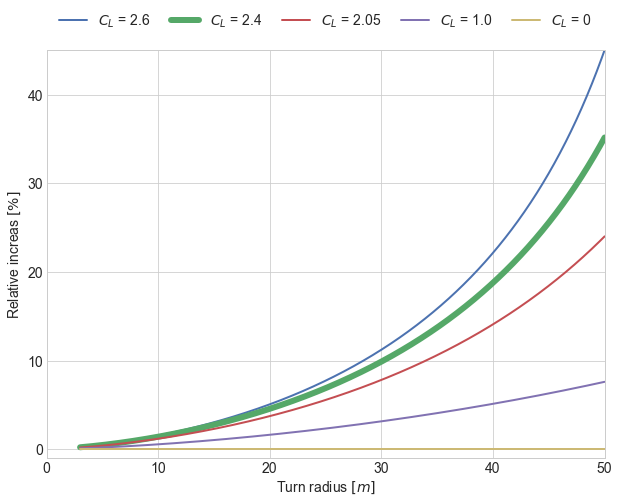
\includegraphics[width=1.2\textwidth]{turnspeedperCLrelative}}%
    \caption{Cornering speed as a function of turn radius for various lift coefficients, relative to a $C_L = 0$.}
    \label{fig:cornerspeedvsliftrelative}
  \end{figure}


  %Based on equation \ref{eq:downforcetocorneringspeed}, the cornering speed due to the added downforce of the wing can be found to give
  %\begin{align}
%    \dot{x} &< \left(\frac{r}{m} \mu (mg + F_L)\right)^{\frac{1}{2}}
%    \intertext{which for a  turn }
%  \end{align}

  While fulfilling the PDS, the ease of prodution and being a first design ever restricted the scope of the project. Great improvements can be expected in the coming years. The extend of the theory required in order to produce a rear wing has been uncovered, and this project serves as a guide line for future iterations of the rear wing.  In chapter \ref{chap:perspective}, a series of possible improvements are evaluated and proposed for increasing the aerodynamic contribution to increasing lap times.
